% arara: pdflatex: { shell: yes }
% arara: biber
% arara: pdflatex: { shell: yes }
% arara: pdflatex: { synctex: true, shell: yes }
%
\documentclass[%
  ,paper=letter
  ,abstract=on
  ,DIV=calc
  ,toc=bib
%  ,twocolumn
%  ,twoside
%  ,BCOR=10mm
%  ,draft
]{scrartcl}

\usepackage{lmodern}

\usepackage[T1]{fontenc}

\usepackage[american]{babel}
\usepackage{csquotes}

\usepackage[babel,final]{microtype}

\usepackage{graphicx}
\graphicspath{{images/}}
\usepackage{epstopdf}

\usepackage{caption}
\usepackage{subcaption}

\usepackage[backend=biber,style=phys,biblabel=brackets,autocite=plain]{biblatex}

\usepackage{filecontents}
\begin{filecontents}{\jobname.bib}
@article{symplectic,
title = "Fourth-order symplectic integration",
journal = "Physica D: Nonlinear Phenomena",
volume = "43",
number = "1",
pages = "105 - 117",
year = "1990",
issn = "0167-2789",
doi = "10.1016/0167-2789(90)90019-L",
url = "http://www.sciencedirect.com/science/article/pii/016727899090019L",
author = "Etienne Forest and Ronald D. Ruth",
}
@book{compphys,
      author        = {Newman, Mark},
      title         = {Computational Physics},
      publisher     = {CreateSpace Independent Publishing},
      address       = {North Charleston, SC},
      year          = {2013},
      isbn = {978148014551},
}
\end{filecontents}
\addbibresource{\jobname.bib}

\usepackage{amsmath, amssymb, amsthm}
\usepackage{amscd}
\usepackage{siunitx}
\sisetup{separate-uncertainty=true, list-final-separator={, and }}
\usepackage{booktabs}
\usepackage{tabularx}
\usepackage{multirow}

\usepackage{authoraftertitle}
\author{Gregory Beauregard}
\title{Final Project}

\usepackage[en-US]{datetime2}
%\date{\today}
\date{\DTMdate{2016-16-23}} % switch to fixed date

\usepackage[hidelinks]{hyperref}
\usepackage[nameinlink,noabbrev,capitalize]{cleveref}

\hypersetup{
  pdftitle   = {\MyTitle},
  pdfauthor  = {\MyAuthor},
  pdfsubject = {Physics}
}

\KOMAoptions{DIV=last}

\begin{document}
\begin{flushright}
\MyAuthor

Computational Physics

Final Project

\MyDate
\end{flushright}

\section{Methods and Background}
\subsection{Problem Conditions}
For my final project I investigated an $n$-body Newtonian gravitational simulation of a merger between two disc galaxies with radial distributions distributed as approximately normal distributions. Each galaxy consisted of 1010 particles, and the initial conditions of the galaxies started them offset by 45 degrees and minimal initial velocity toward each other. In these galaxies each particle had the same mass with the exception of a black hole in the center of each galaxy with a mass of 10 particles. The force was calculated using the relation
\begin{equation}
\mathbf{F}_{ij}=\frac{\mathbf{q}_j-\mathbf{q}_i}{\left(\lVert \mathbf{q}_j-\mathbf{q}_i\rVert^2+\varepsilon\right)^{3/2}}.
\end{equation}
In my code I used $\varepsilon=0.01$. This serves to soften the potential to remove the ability of the particles in the simulation to form tight binaries which are unphysical when the particles are meant to represent many stars in a disc galaxy which, individually, do not pass close.

\subsection{Accuracy}
In order to address the issue of simulation accuracy over long periods of time, a symplectic integrator was used. After exploring several options, I implemented a fourth order symplectic integrator following the approach given by Ruth \autocite{symplectic}.

In order to verify the accuracy and symplectic property of the integrator I programmed, the convergence and energy tests of HW 5 were re-run using the 4th order symplectic integrator. The results are shown in \cref{fig:q1:plot}.

\begin{figure}[h!]
\centering
\begin{subfigure}[t]{0.495\textwidth}
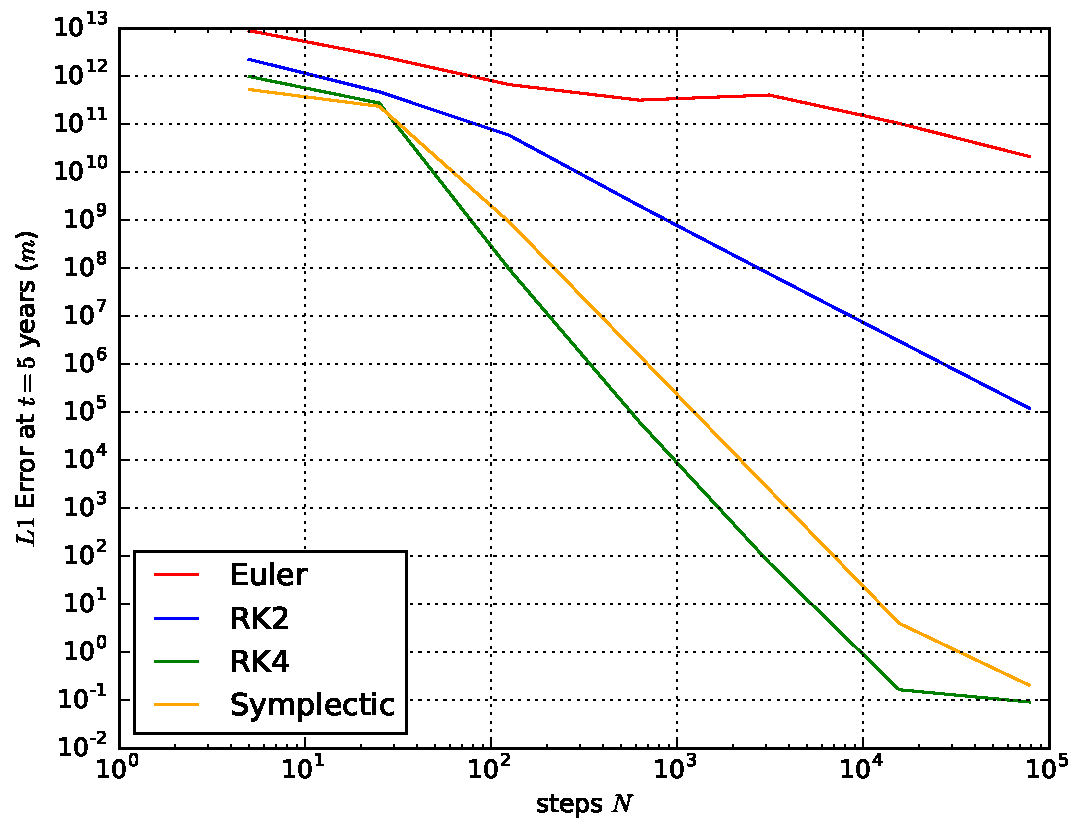
\includegraphics[width=\textwidth,keepaspectratio]{1_error}
\caption{$L_1$ error of mars evolution}
\label{fig:one}
\end{subfigure}
\begin{subfigure}[t]{0.495\textwidth}
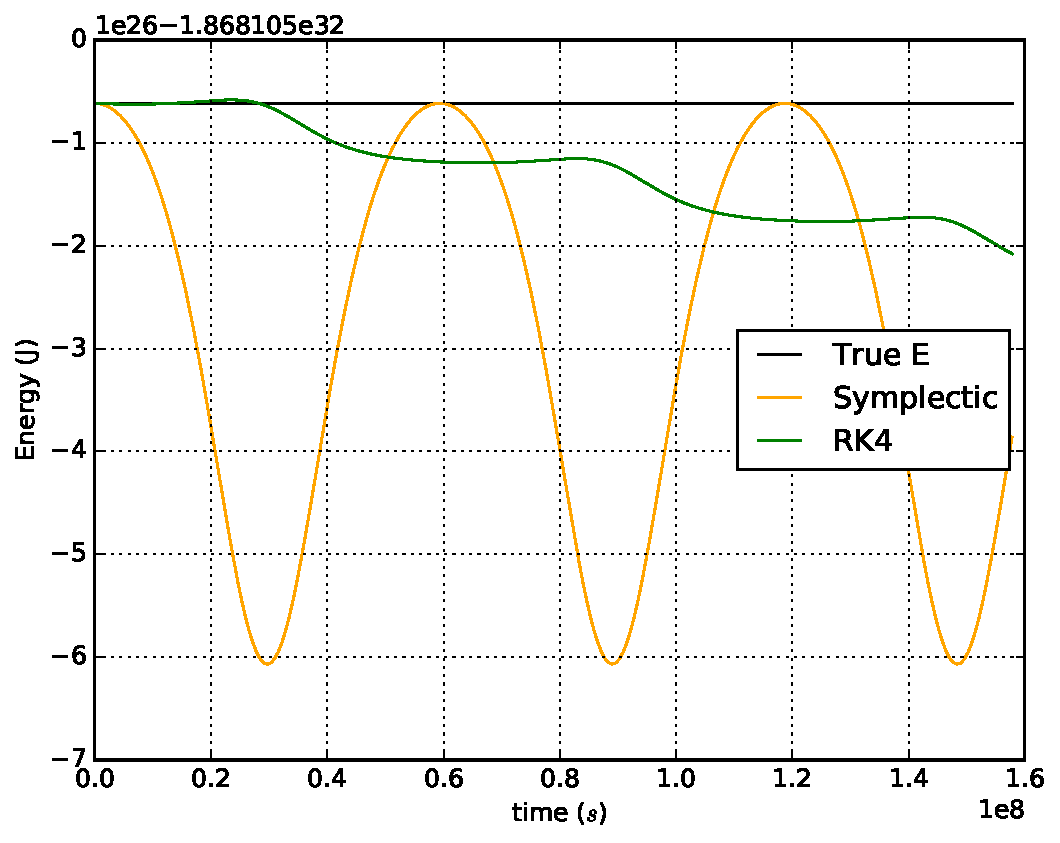
\includegraphics[width=\textwidth,keepaspectratio]{1_rk4_energy}
\caption{Energy conservation over time}
\label{fig:two}
\end{subfigure}
\caption{Plots demonstrating the difference between integrators with respect to convergence and energy conservation.}
\label{fig:q1:plot}
\end{figure}

As demonstrated by \cref{fig:q1:plot}, the code is nearly as good as RK4 while still conserving energy.

\subsection{Performance}
Another major issue encountered during the project was performance. Since the needed to be able to support several thousand particles, I found Python loops to be much too slow. To get around issues with Python's performance, the force calculation between each particle was done entirely in \texttt{numpy}. Although this improved performance significantly, performance was still below what I had hoped. To further increase the performance, I loaded and used parallelized computational libraries that were able to do operations on numpy arrays parallelized across CPU cores. After implementing this code in the \texttt{solve.py} file, the performance was improved enough to be able to run the simulation.

\section{Results and Conclusion}
The resulting simulation was saved to disc as hdf5 and then rendered to video for upload to \href{https://www.youtube.com/watch?v=Qp0M3gj23YY}{YouTube (click)}. The simulation depicts a head-on collision in which the galaxies first appear to pass through each other before quickly falling back in on themselves several times. As the two original galaxy cores become locked the particles all begin to orbit the core in apparently random orientations and eccentricities; this is an elliptical galaxy. This is an excellent result because it is well accepted that similar sized merging disc galaxies will form elliptical galaxies.

Several interesting things to explore from here would be the development of spiral arms in galaxies and the effect of dark matter on galactic evolution.

\printbibliography

\end{document}